\ProvidesFile{ch-light-curve-simulation.tex}[Light Curve Simulation]
\graphicspath{{/Users/liamrobinson/Documents/PyLightCurves/docs/build/html/_images}}

\section{Light Curve Simulation}

\subsection{Orbital Dynamics}

TODO

\subsection{Discrete Shape Representations}

A computer can represent 3D objects implicitly or explicitly. An implicit representation might be the solution to an algebraic equation, i.e., $x^2 + y^2 + z^2 = 1$ defines a sphere of radius $1$ centered at the origin. Often, a shape may be defined by a set of signed distance functions (SDFs). An SDF takes in a point in \rthree and outputs the distance from the object, returning negative distance if the queried point is inside the shape. The object can then be rendered via ray marching. A ray is cast from the camera out into the scene for each pixel of the screen, each performing distance queries along its length until it intersects the object or diverges. 

By contrast, an explicit shape representation creates complex 3D geometry from simple 2D building blocks. In the most common case, object faces are defined by triangles. This means that at the scale of the individual faces, the shape is always composed of flat surfaces that meet at sharp angles. While this can add complexity to many fields of shape analysis and geometry processing, triangulated surfaces are perfect for our application. Human-made space objects like most satellites are composed of flat faces, with the exception of parabolic antennas and cylindrical rocket bodies.

\subsubsection{The Object File Format}

One common text file format for 3D model files is \texttt{.obj}, developed by Wavefront Technologies in the early 1990s \cite{obj_format}. Each OBJ file consists of a list of vertex positions and face definitions, with optional vertex normals and tangents. An \texttt{.obj} listing for a cube is included for reference in Appendix \ref{sec:obj_listing}. Given the vertex positions and adjacency information stored in the model file, useful properties of the object can be computed for use later in both light curve simulation and shape inversion. For each triangular face $F_i$ of the model defined by vertices $F_i = \left\{v_1, v_2, v_3\right\}$, the outward-pointing face normal is computed with

\begin{equation} \label{eq:face_normal}
    \hat{n} = \frac{\left( v_2 - v_1 \right) \times \left( v_3 - v_1 \right)}{\| \left( v_2 - v_1 \right) \times \left( v_3 - v_1 \right) \|_2}.
\end{equation}

The face area is computed with

\begin{equation} \label{eq:face_areas}
    a = \frac{\| \left( v_2 - v_1 \right) \times \left( v_3 - v_1 \right)\|_2}{2}.
\end{equation}

The support of each face --- the perpendicular distance from the origin to the plane defining the face --- is computed with

\begin{equation} \label{eq:face_support}
    h = v_1 \cdot \hat{n}.
\end{equation}

The volume of the entire object is compute with

\begin{equation} \label{eq:object_volume}
    \frac{1}{3} \sum_{i=0}^{ \lvert F \rvert}\vec{h}_i \cdot \vec{a}_i.
\end{equation}

In Eq \ref{eq:object_volume}, $\lvert F \rvert$ is the number of faces defining the object. $\vec{h}$ and $\vec{a}$ are column vectors collecting all face supports and areas. The Extended Gaussian Image, a quantity defined in \ref{sec:egi_definition}, is computed row-wise for the $i$th face with

\begin{equation} \label{eq:egi_definition}
    \vec{E}_i = \vec{a}_i \vec{n}_i.
\end{equation}

\subsection{Selected Satellite Models}

Most of the analysis in this work used one of the 3D model files shown in Figure \ref{fig:satellite_lineup}. Figure \ref{fig:satellite_lineup} highlights the size of the GEO communications satellites (TELSTAR, HYLAS, Hispasat, and ASTRA). In contrast, the LEO satellites (Starlink and Landsat) are dwarfed at the left end of the lineup.

\begin{figure}[ht]
    \centering
    \includegraphics[width=\figbig]{sphx_glr_satellite_lineup_001.png}
    \caption{Selected space objects with soccer field for size reference. In order, the objects are TESS, Starlink V1, TDRS, Landsat 8, Hispasat 30W-6, Saturn V SII, TELSTAR 19V, HYLAS 4, and simplified ASTRA.
    }
    \label{fig:satellite_lineup}
\end{figure}

\subsection{The Bidirectional Reflectance Distribution Function}

Although light curves come from unresolved measurements, the interactions that produce them are directly driven by the shape and material properties of the object being observed. In order to simulate accurate light curves, all relevant optical interactions must be modeled. In broad terms, this boils down to determining how the object is illuminated, how it casts shadows on itself, and how it is observed. 

At the microscopic scale, the surface of an object is composed of facets ---  small areas sharing a normal vector. The macroscopic optical properties of the material is driven by the distribution of sizes and normal directions of these microfacets. If the facet normals are distributed in biased orientations, the macroscopic surface may show anisotropy, leading to the appearance of brushed metal. If the facets normals are at large angles to each other, the surface may appear dull as the direction of the outgoing light may be largely independent from the incoming direction. Subsurface effects ---  where incoming light rays scatter \textit{inside} the surface can also change the macroscopic properties of the material. 

This discussion raises an important question; how should the macroscopic outcomes of the microscopic interactions of incident light on a surface be modeled? The bidirectional reflectance distribution function (BRDF) is a tool from computer graphics that addresses this problem. The BRDF is a function on the hemisphere which expresses the fraction of light per solid angle (radiance $\mathcal{R}$) leaving the surface in a given direction, divided by the incident power per unit area (irradiance $\mathcal{I}$). The general formulation for a BRDF $f_r$ is given by Eq \ref{eq:brdf_def} \cite{duvenhage2013}.

\begin{equation}
    f_r(\vctr{x}, L \rightarrow O) = \frac{d\mathcal{R}\left(\vctr{x} \rightarrow O\right)}{d\mathcal{I}\left(L \rightarrow \vctr{x}\right)}
    \label{eq:brdf_def}
\end{equation}

In Eq \ref{eq:brdf_def}, $\vctr{x} \in \mathbb{R}^3$ is the point on the object's surface where the BRDF is evaluated. $L \in \mathbb{S}^2$ is the incoming illumination unit vector and $O \in \mathbb{S}^2$ is the outgoing unit vector. Note that this work treats $f_r(\vctr{x}, L \rightarrow O)$ and $f_r(L \rightarrow O)$ as equivalent in later descriptions, leaving the evaluation point $\vctr{x}$ implied. This definition is useful for building intuition about the form of the BRDF, but to represent a physically plausible reflection process, a candidate function must satisfy three additional constraints. A physically plausible BRDF must conserve energy --- more energy cannot be reflected from the surface than was incident on it. It must also be reciprocal --- switching the observer and illumination directions should not change the BRDF value as the surface interaction. This reciprocity is sometimes known as the \textit{Helmholtz Reciprocity Rule} in literature \cite{montes2012}. Finally, plausible BRDFs are positive --- they take on nonnegative values for all valid inputs \cite{montes2012}. A surface cannot reflect negative light, so this should feel natural. Explicitly, energy conservation is expressed by Eq \ref{eq:brdf_energy_cons} \cite{montes2012}.

\begin{equation} \label{eq:brdf_energy_cons}
  \forall L \in \mathbb{S}^2 : \:\: \int_{O \in \mathbb{S}^2} f_r(L \rightarrow O) \: d\mathbb{S}^2 \leq 1
\end{equation}

Eq \ref{eq:brdf_energy_cons} states that for all possible illumination directions $L$, integrating all possible outgoing observer directions $O$ on the unit sphere cannot return greater than one from the energy conservation integral. Reciprocity can also be formalized via \ref{eq:brdf_reciprocity}.

\begin{equation} \label{eq:brdf_reciprocity}
  \forall L, O \in \mathbb{S}^2 : \:\: f_r(L \rightarrow O) = f_r(O \rightarrow L)
\end{equation}

\subsection{BRDF Formulations}

Now that the requirements for a plausible physical BRDF have been established, a collection of commonly-used BRDFs can be presented. The following BRDFs are all energy conserving, reciprocal, and nonnegative. \textit{Caveat emptor}: this does not mean that they are always sufficient for modeling real-world materials, they merely represent ways hypothetical surfaces could reflect light without breaking any fundamental physics.

\subsubsection{Lambertian}

The simplest BRDF is one that reflects equally in all directions. This BRDF is termed Lambertian or diffuse.

\begin{equation} \label{eq:brdf_lambertian}
  f_r(L \rightarrow O) = \frac{C_d}{\pi}
\end{equation}

In Eq \ref{eq:brdf_lambertian}, $0 \leq C_d \leq 1$ is the surface's coefficient of diffuse reflection. For example, $C_d = 0.4$ means that the surface reflects $40\%$ of incident radiation and absorbs the other $60\%$. 

\subsubsection{Phong}

While the diffuse BRDF reflects energy isotropically, many real-world reflections are highly biased. At the extreme end, a perfect mirror reflection is effectively a Dirac delta function in the reflected illumination direction. Many real-world materials are well-modeled as a linear combination of diffuse and specular effects. A simple specular BRDF model is that developed by Phong in 1975 \cite{phong1975}. The Phong model splits the BRDF into a Lambertian term governed by $C_d$ and a specular term governed the coefficient of specular reflection $ 0 \leq C_s \leq 1$ and the specular exponent $n \geq 0$ \cite{duvenhage2013}. 

\begin{equation} \label{eq:brdf_phong}
  f_r(L \rightarrow O) = \frac{C_d}{\pi} + \frac{C_s \frac{n+2}{2\pi} (O \cdot R)^n}{N \cdot L}
\end{equation}

In Eq \ref{eq:brdf_phong}, $R$ is the reflected illumination vector, computed via $R = 2 (N \cdot L) N - L$. As $n$ increases, the specular glint becomes sharper and more intense, eventually approaching a perfectly mirror reflection. Because of the introduction of a new coefficient of reflection, a new constraint is needed to maintain energy conservation. Because $C_d$ and $C_s$ each represent the \textit{fraction} of light reflected in each mode, it should be clear that $C_d + C_s \leq 1$. This can also be reformulated with an explicit coefficient of absorption $C_a$ which captures the fraction of incident radiation absorbed by the surface, yielding $C_d + C_s + C_a = 1$. 

\subsubsection{Blinn-Phong}

The Blinn-Phong BRDF is similar to to the Phong BRDF, but parameterizes the specular lobe in terms of the halfway vector $H$ \cite{duvenhage2013}. This vector is halfway between the illumination and observer directions such that $H = L + O$ which needs to be normalized before use. As the halfway vector approaches the surface normal vector, the observer must be approaching the reflected illumination vector, leading to a more intense specular highlight. 

\begin{equation} \label{eq:brdf_blinn_phong}
  f_r(L \rightarrow O) = \frac{C_d}{\pi} + \frac{C_s \frac{n+2}{2\pi} (N \cdot H)^n}{4 (N \cdot L)(N \cdot O)}
\end{equation}

\subsubsection{Glossy}

TODO

\subsubsection{Cook-Torrance}

TODO

\subsubsection{Oren-Nayar}

TODO

\subsubsection{Ashikhmin-Shirley}

TODO

\subsection{BRDF Summary}

\begin{figure}[ht]
  \includegraphics[width=\figmed]{sphx_glr_brdf_renders_002_2_00x.png}
  \caption
  {Implemented BRDFs rendered with arbitrary parameters, demonstrating the qualitative differences between lighting models}
  \label{fig:brdf_renders}
\end{figure}

\subsection{Simulating Light Curves for Convex Objects}

Light curve simulation for convex geometry can be solved semi-analytically as each face's contribution 
to the measured irradiance can be computed individually \cite{kaasalainen2001}. 
Determining whether a face is illuminated requires two horizon checks to determine visibility 
from the Sun and to the observer. For a face $i$ at timestep $j$ these horizon checks are 
expressed by the shadowing condition $\mu_{ij}$. 

\begin{equation} \label{eq:cvx_shadow_cond}
  \mu_{ij} = \begin{cases}
    1 \text{ if } \left( O_j \cdot \hat{n}_i \right) > 0 \text{ and } \left( L_j \cdot \hat{n}_i \right) > 0 
	  \text{ and } \delta_{ij,\text{ss}} = 0 \text{ and } \delta_{ij,\text{os}} = 0\\
    0 \text{ otherwise } \\
  \end{cases}
\end{equation}

The unit vectors $O$ and $L$ point from the center of mass of the object to the observer and Sun, respectively. 
We choose the outward-pointing face normal unit vector $\hat{n}$ by convention for all mesh operations. 
The self-shadowing and observer-shadowing conditions, $\delta_{ij,\text{ss}}$ and $\delta_{ij,\text{os}}$, 
are always zero for convex polyhedra but are crucial for accurately simulating non-convex geometry. 
For objects with concavities, self-shadowing refers to shadows cast by an object onto itself and observer-shadowing 
refers to otherwise visible faces blocked by other portions of the geometry.

The irradiance $I$ received by the observer at timestep $j$ is the sum of the received irradiance from all faces, 
composed of specular and diffuse contributions. Each contribution is expressed as the product of the
normalized irradiance $\hat{I}$. This can be scaled to adjust for the distance from the observer to
the object to yield the noiseless received irradiance.

TODO: add L = Ga stuff

\subsection{Simulating Light Curves for Non-Convex Objects}

Many existing light curve simulation methods for non-convex objects rely on ray tracing schemes like Möller and Trumbore's ray-triangle intersection algorithm \cite{moller2005,fan2020thesis}. This computation has complexity $\mathcal{O}(n^2)$ if implemented naïvely, but can be improved to $\mathcal{O}(n \ln n)$ with better spatial data structures. For human-made space objects, there may be significant self-shadowing at large phase angles. As a result, it cannot be assumed that the self-shadowing conditions $\delta_{ij,\text{ss}}$ and $\delta_{ij,\text{os}}$ are zero \cite{frueh2014,fan2020thesis}. Naïve ray traced shadows generally require $\mathcal{O}(n^2)$ ray-triangle intersections per timestep for $n$ faces. For this reason, ray traced shadows quickly become infeasible for complex objects without GPU parallelization. The limitations of ray-triangle intersections for light curve simulation is discussed at length by Frueh et al. \cite{frueh2014}.

\graphicspath{{/Users/liamrobinson/Documents/msthesis/static_images/aas_2022_figs}}
\begin{figure}[!htb]
  \centering
  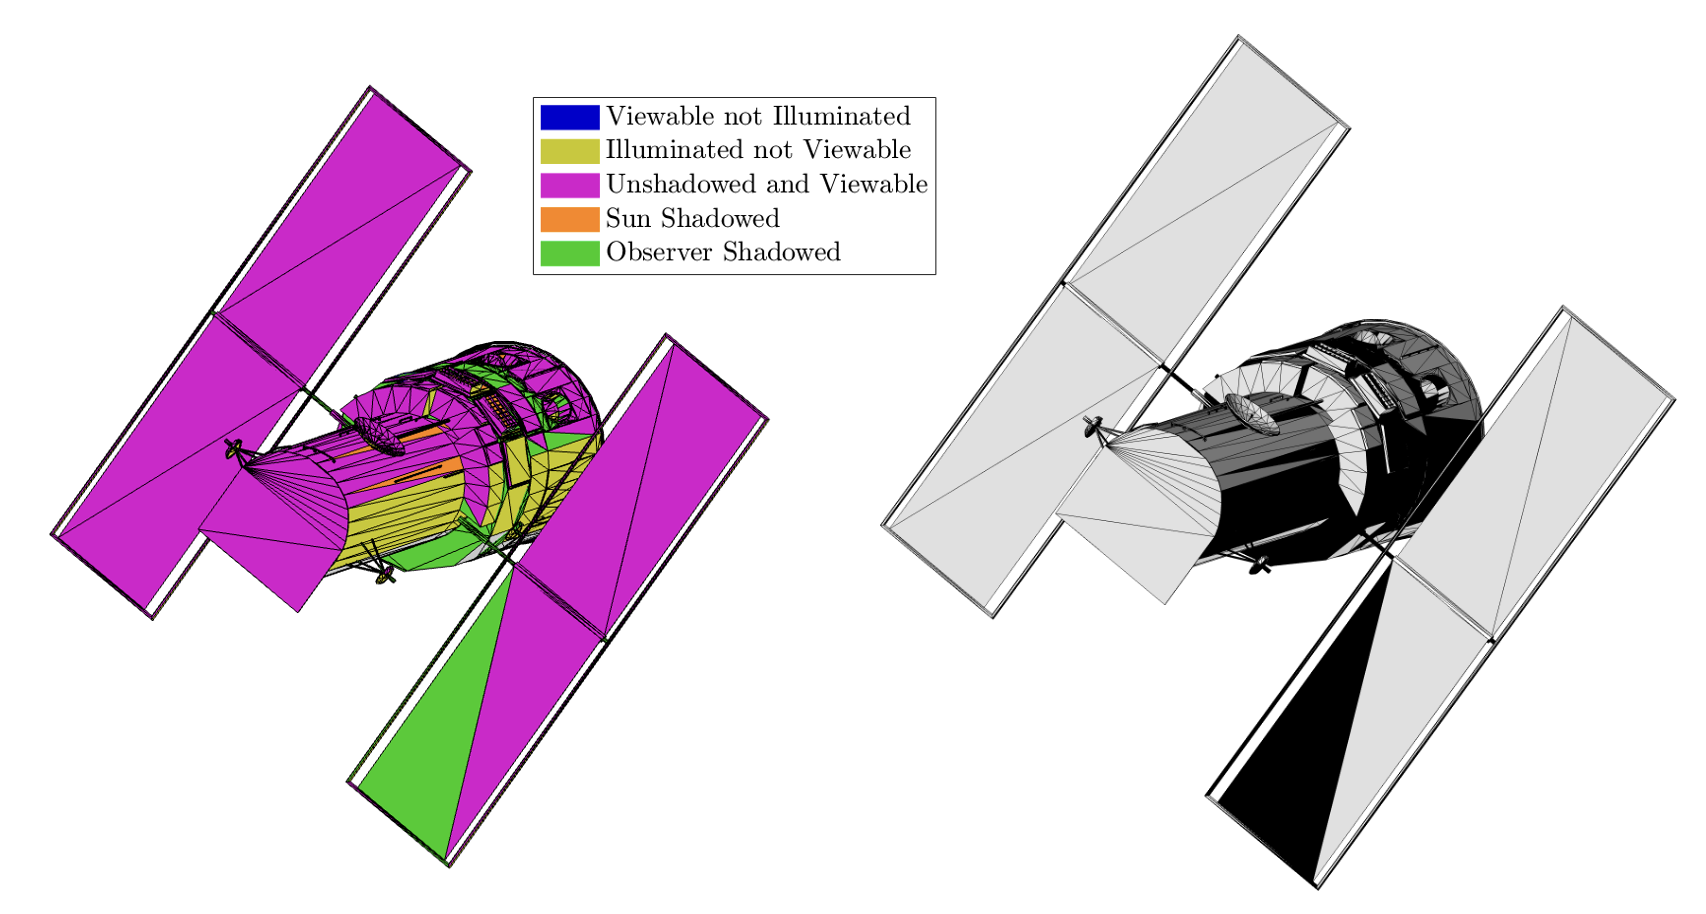
\includegraphics[width=350px]{hst_shadow_mapping/composite_hst_raytraced.png}
  \caption{Hubble Space Telescope ray traced shadow categorization and shading. Models from \cite{nasa_models}}
  \label{hst_shadows_ray}
\end{figure}

\subsection{The Importance of Self-Shadowing}

To motivate the need for accurate shadows when dealing with human-made space objects, consider the error introduced by neglecting shadows for different types of space objects. Kaasalainen and Torppa's work on asteroids reasonably assumed that shadowing was a negligible contribution to the measured light curve. Human-made objects do not afford the same luxury. Figure \ref{fig:hst_bennu_shadows} displays light curves for the asteroid Bennu and the Hubble Space Telescope with and without accurate shadows under a single-axis spin profile with inertially fixed Sun and observer vectors. Without accurate shadowing, the light curve's intensity and its time derivative can be significantly error-prone.

\begin{figure}[!htb]
  \centering
  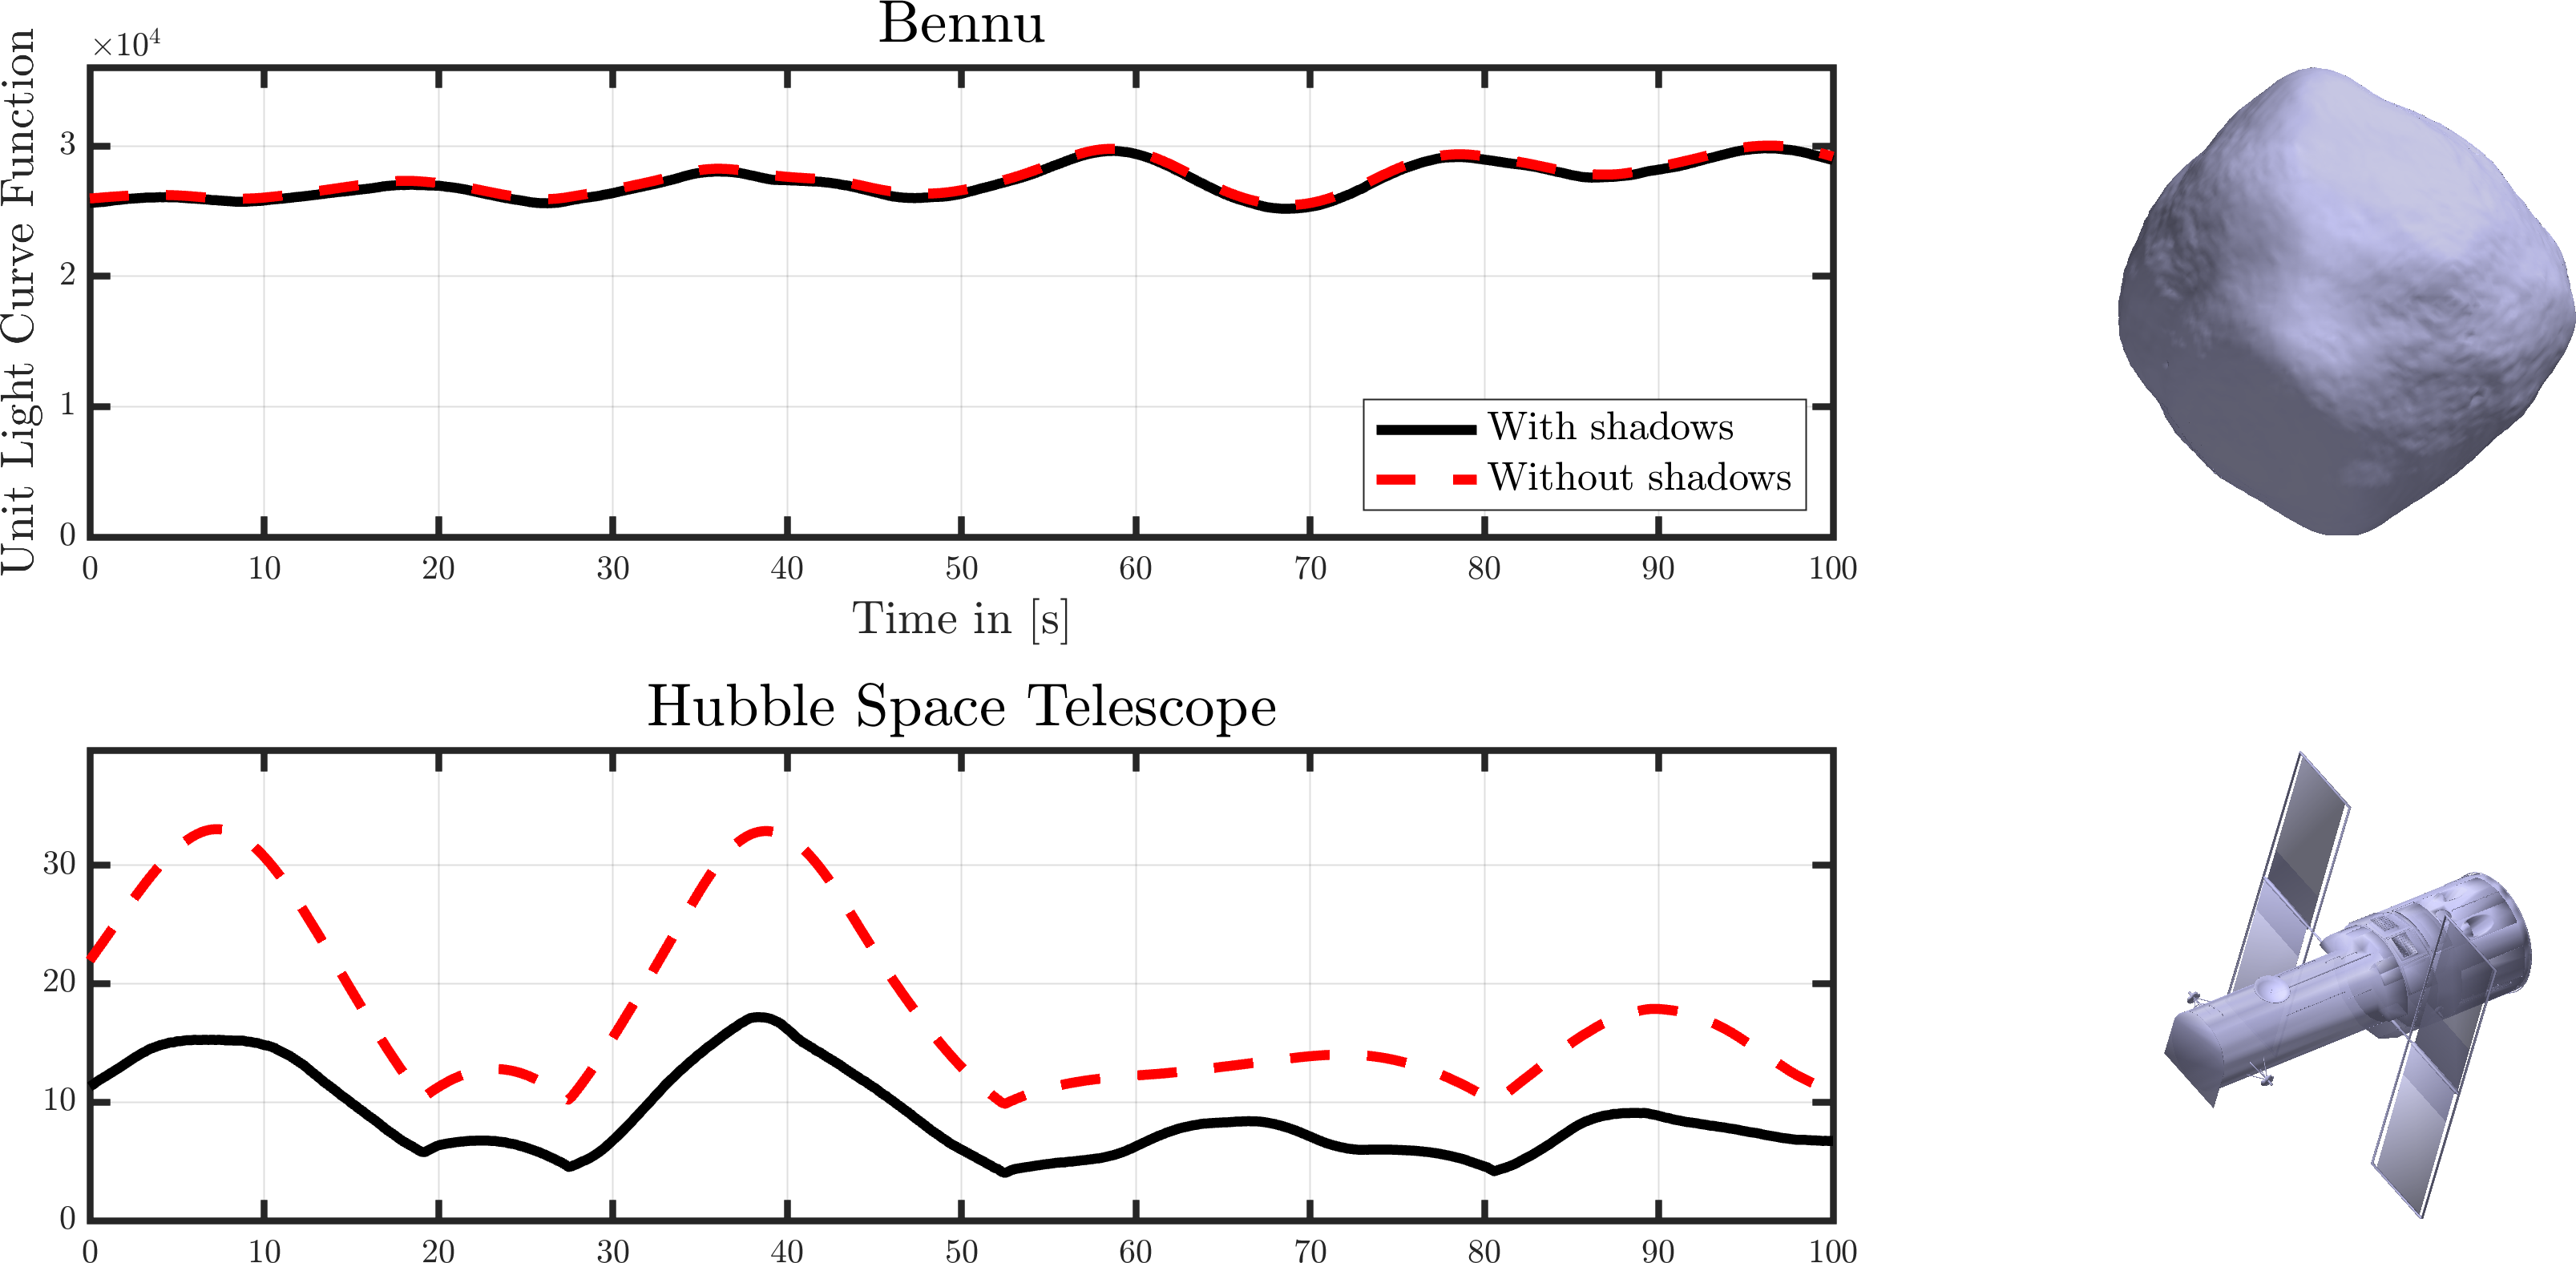
\includegraphics[width=350px]{convex_vs_nconv_lcs.png}
  \caption{Brightness errors introduced by neglecting shadows for Bennu and HST. Models from \cite{nasa_models}}
  \label{fig:hst_bennu_shadows}
\end{figure}

\subsection{Shadow Mapping}

\begin{figure}[!htb]
  \centering
  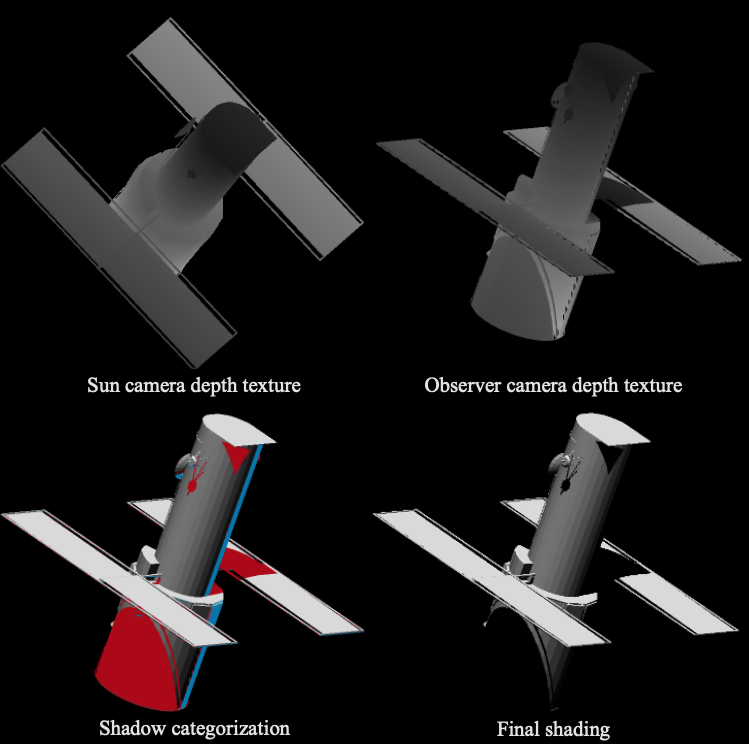
\includegraphics[width=200px]{hst_shadow_mapping/hst_shadow_mapping.png}
  \caption{Hubble Space Telescope shadow mapping with self (red) and horizon (blue) shadows rendered. Models from \cite{nasa_models}}
  \label{fig:hst_shadows_map}
\end{figure}

TODO: remake \ref{fig:hst_shadows_map} with figure from Python.

In the LightCurveEngine, shadow mapping is used for faster and more accurate self-shadowing. Shadow mapping is a well understood technique in computer graphics \cite{kolivand2013}. Although modern ray traced shadowing may be more computationally efficient, shadow mapping was selected for its ease of implementation \cite{kolivand2013}. Because shadow mapping shades individual pixel fragments instead of entire faces, it offers increasing shadow quality over facewise ray tracing as the number of mesh faces falls.

Given an observer and Sun vector in the body frame of the object, shadow mapping proceeds in a four step process. In step one, a camera is positioned along the Sun vector and a perpendicular depth texture is computed. In the second step, depth values in Sun camera space are transformed to observer camera space, where a second depth texture is computed. This second texture is used to find the closest fragment along each ray to the Sun \cite{brabec2002}. Self-shadowed fragments are classified as those further from the Sun than the closest fragment along the same ray, indicated in red in Figure \ref{fig:hst_shadows_map}. Fragments that do not pass the convex shadowing condition are horizon shadowed, indicated in blue in Figure \ref{fig:hst_shadows_map}, determining the Sun and observer shadowing conditions at once. All remaining fragments are shaded with using the same Lambertian reflection model in \ref{eq:lc_func_diffuse} TODO: this equation is broken. Computing the light curve function for the final rendered image requires summing all pixel values and dimensionalizing the result by the area of the observer camera's field of view. The light curve simulation environment used in this work was implemented in C and OpenGL using raylib \cite{raylib}.

TODO: add algorithm pseudocode for lighting shader

\subsection{Sampling Noisy Light Curves}

Given the irradiance of the object observed by the telescope, the noisy light curve is computed by building a grid containing the object signal, background noise, and sensor noise. On a pixel-by-pixel basis, the mean object signal is given by an alteration of Eq \ref{eq:airy_gaussian}:

\begin{equation} \label{eq:obj_signal_grid}
  C_{obj}(x, y) = \frac{0.838 \bar{C}_{all}}{2 \pi \sigma^2} \exp\left( - \frac{(x - x_0)^2 + (y - y_0)^2}{2 \sigma^2  s_{pix}^2} \right).
\end{equation}

In Eq \ref{eq:obj_signal_grid}, $\left(x_0, y_0\right)$ are the exact pixel coordinates of the object centroid, $\sigma$ is the Gaussian standard deviation from Eq \ref{eq:airy_variance} in arcseconds, and $s_{pix}$ is the pixel scale in arcseconds per pixel. Likewise, the total noise sampled in each pixel is given by samples from all the relevant source distributions:

\begin{equation} \label{eq:noise_signal_grid}
  C_{noise}(x, y) = N_{background} + N_{dark} + N_{trunc} + N_{read}.
\end{equation}

In Eq \ref{eq:noise_signal_grid}, $N_{background}$ is a sample drawn from $\mathrm{Pois}(\lambda_{background})$, $N_{dark}$ is drawn from $\mathrm{Pois}(\Delta t \lambda_{dark})$, $N_{trunc}$ is drawn from $\mathrm{Uniform}(-g/2, g/2)$, and $N_{read}$ is drawn from $\mathrm{Normal}(0, \sigma_{read}^2)$. 